\chapter{Camera calibration}

\begin{description}
    \item[World reference frame (WRF)] \marginnote{World reference frame (WRF)}
        Coordinate system $(X_W, Y_W, Z_W)$ of the real world relative to a reference point (e.g. a corner).

    \item[Camera reference frame (CRF)] \marginnote{Camera reference frame (CRF)}
        Coordinate system $(X_C, Y_C, Z_C)$ that characterizes a camera.

    \item[Image reference frame (IRF)] \marginnote{Image reference frame}
        Coordinate system $(U, V)$ of the image.
        They are obtained as a perspective projection of CRF coordinates as:
        \[ 
            u = \frac{f}{z}x_C 
            \hspace{3em} 
            v = \frac{f}{z}y_C 
        \]

    \begin{figure}[H]
        \centering
        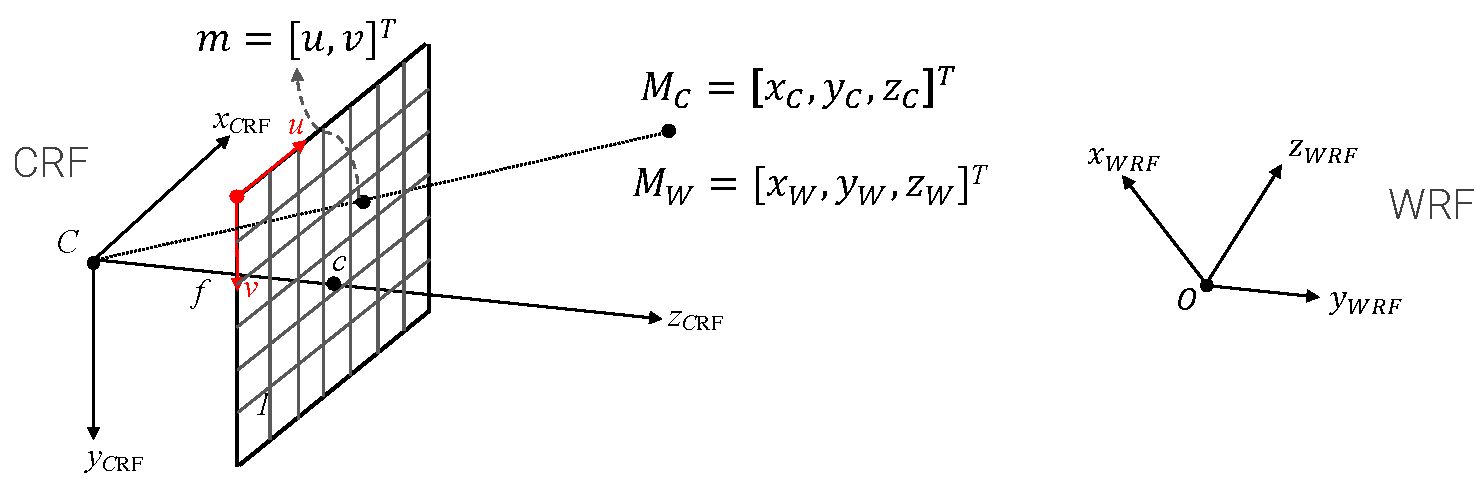
\includegraphics[width=0.8\linewidth]{./img/_formation_system.pdf}
        \caption{Example of WRF, CRF and IRF}
    \end{figure}
\end{description}



\section{Forward imaging model}


\subsection{Image pixelization (CRF to IRF)}
\marginnote{Image pixelization}

The conversion from the camera reference frame to the image reference frame
is done in two steps:
\begin{descriptionlist}
    \item[Discetization] \marginnote{Discetization}
        Given the sizes (in mm) $\Delta u$ and $\Delta v$ of the pixels,
        it is sufficient to modify the perspective projection to map CRF coordinates into a discrete grid:
        \[ 
            u = \frac{1}{\Delta u}\frac{f}{z_C}x_C 
            \hspace{3em} 
            v = \frac{1}{\Delta v}\frac{f}{z_C}y_C 
        \]

    \item[Origin translation] \marginnote{Origin translation}
        To avoid negative pixels, the origin of the image has to be translated from the piercing point $c$ to the top-left corner.
        This is done by adding an offset $(u_0, v_0)$ to the projection (in the new system, $c = (u_0, v_0)$):
        \[ 
            u = \frac{1}{\Delta u}\frac{f}{z_C}x_C + u_0
            \hspace{3em} 
            v = \frac{1}{\Delta v}\frac{f}{z_C}y_C +v_0
        \]

    \begin{figure}[H]
        \centering
        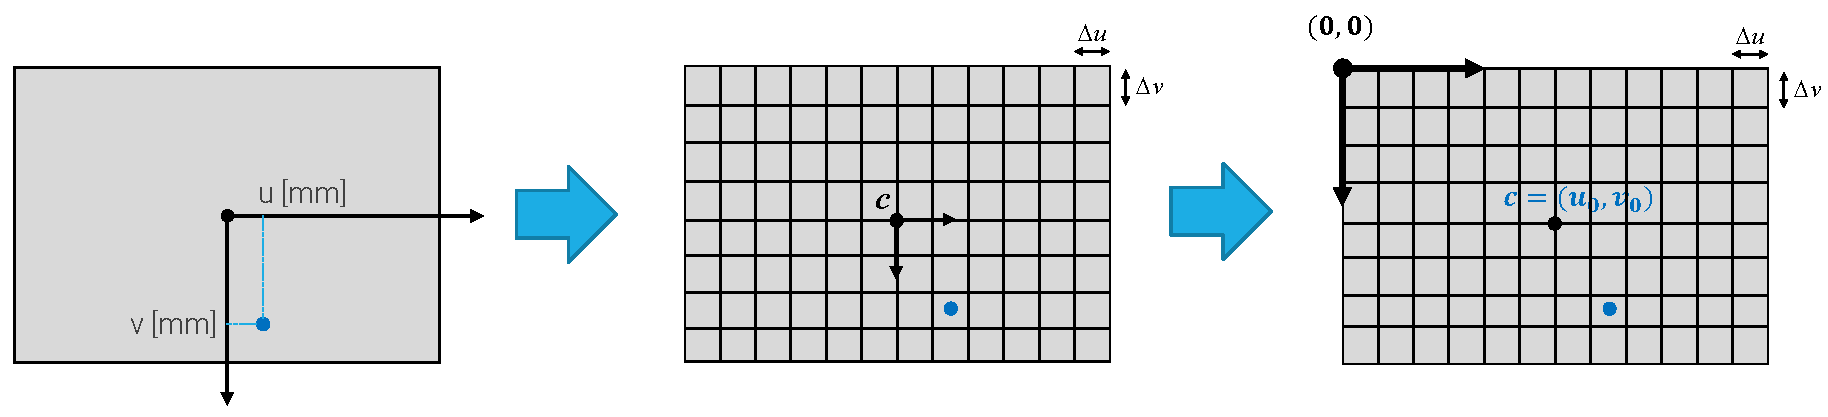
\includegraphics[width=0.9\linewidth]{./img/_pixelization.pdf}
        \caption{Pixelization process}
    \end{figure}

    \item[Intrinsic parameters] \marginnote{Intrinsic parameters}
        Parameters needed to convert from CRF to IRF.

        By fixing $f_u = \frac{f}{\Delta u}$ and $f_v = \frac{f}{\Delta v}$, the projection can be rewritten as:
        \[ 
            u = f_u\frac{x_C}{z_C} + u_0
            \hspace{3em} 
            v = f_v\frac{y_C}{z_C} +v_0
        \]
        Therefore, there is a total of 4 parameters: $f_u$, $f_v$, $u_0$ and $v_0$.
\end{descriptionlist}


\subsection{Roto-translation (WRF to CRF)}
\marginnote{Roto-translation}

The conversion from the world reference system to the camera reference system
is done through a roto-translation wrt the optical center.

Given: 
\begin{itemize}
    \item A WRF point $\vec{M}_W = (x_W, y_W, z_W)$,
    \item A rotation matrix $\matr{R}$,
    \item A translation vector $\vec{t}$,
\end{itemize}
the coordinates $\vec{M}_C$ in CRF corresponding to $\vec{M}_W$ are given by:
\[  
    \vec{M}_C = \begin{pmatrix} x_C \\ y_C \\ z_C \end{pmatrix} =
    \matr{R}\vec{M}_W + \vec{t} =
    \begin{pmatrix}
        r_{11} & r_{12} & r_{13} \\
        r_{21} & r_{22} & r_{23} \\
        r_{31} & r_{32} & r_{33} \\
    \end{pmatrix}
    \begin{pmatrix}
        x_W \\ y_W \\ z_W
    \end{pmatrix}
    +
    \begin{pmatrix}
        t_1 \\ t_2 \\ t_3
    \end{pmatrix}
\]

\begin{remark}
    The coordinates $\vec{C}_W$ of the optical center $\vec{C}$ are obtained as:
    \[ 
        \nullvec = \matr{R}\vec{C}_W + \vec{t} 
            \iff (\nullvec - \vec{t}) = \matr{R}\vec{C}_W 
            \iff \vec{C}_W = \matr{R}^T (\nullvec - \vec{t})
            \iff \vec{C}_W = -\matr{R}^T\vec{t}
    \]
\end{remark}

\begin{description}
    \item[Extrinsic parameters] \marginnote{Extrinsic parameters}
        \phantom{}
        \begin{itemize}
            \item The rotation matrix $\matr{R}$ has 9 elements of which 3 are independent (i.e. the rotation angles around the axes). 
            \item The translation matrix $\vec{t}$ has 3 elements.
        \end{itemize}

        Therefore, there is a total of 6 parameters.
\end{description}


\begin{remark}
    It is not possible to combine the intrinsic camera model and the extrinsic roto-translation to
    create a linear model for the forward imaging model.
    \[
        u = f_u \frac{r_{11}x_W + r_{12}y_W + r_{13}z_W + t_1}{r_{31}x_W + r_{32}y_W + r_{33}z_W + t_3} + u_0
        \hspace{1.5em}
        v = f_v \frac{r_{21}x_W + r_{22}y_W + r_{23}z_W + t_2}{r_{31}x_W + r_{32}y_W + r_{33}z_W + t_3} + v_0
    \]
\end{remark}



\section{Projective space}

\begin{remark}
    In the 2D Euclidean plane $\mathbb{R}^2$, parallel lines never intersect and points at infinity cannot be represented.
    \begin{figure}[H]
        \centering
        \begin{subfigure}{0.45\linewidth}
            \centering
            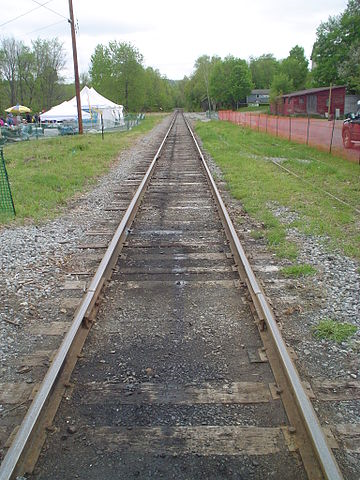
\includegraphics[width=0.45\linewidth]{./img/point_infinity_example1.png}
        \end{subfigure}
        \begin{subfigure}{0.45\linewidth}
            \centering
            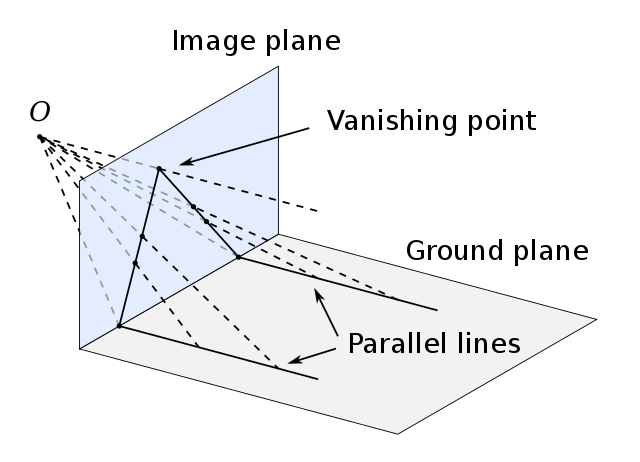
\includegraphics[width=0.8\linewidth]{./img/point_infinity_example2.png}
        \end{subfigure}
        \caption{Example of point at infinity}
    \end{figure}
\end{remark}

\begin{remark}
    Point at infinity is a point in space while the vanishing point is in the image plane.
\end{remark}

\begin{description}
    \item[Homogeneous coordinates] \marginnote{Homogeneous coordinates}
        Without loss of generality, consider the 2D Euclidean space $\mathbb{R}^2$.

        Given a coordinate $(u, v)$ in Euclidean space, its homogeneous coordinates have an additional dimension
        such that:
        \[ (u, v) \equiv (ku, kv, k) \,\forall k \neq 0 \]
        In other words, a 2D Euclidean point is represented by an equivalence class of 3D points.

    \item[Projective space] \marginnote{Projective space}
        Space $\mathbb{P}^n$ associated with the homogeneous coordinates of an Euclidean space $\mathbb{R}^n$.

        \begin{figure}[H]
            \centering
            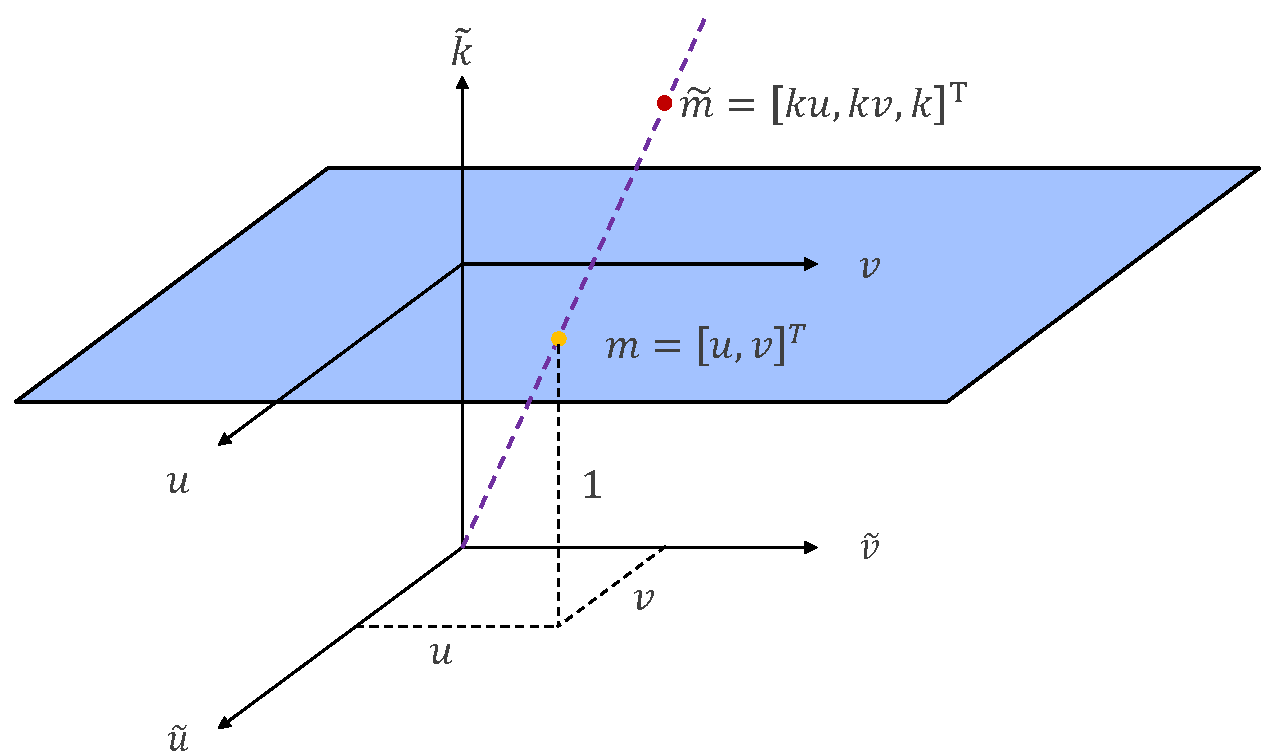
\includegraphics[width=0.6\linewidth]{./img/_projective_space.pdf}
            \caption{Example of projective space $\mathbb{P}^2$}
        \end{figure}

        \begin{remark}
            $\nullvec$ is not a valid point in $\mathbb{P}^n$.
        \end{remark}

        \begin{remark}
            A projective space allows to homogeneously handle both ordinary (image) and ideal (scene) points without introducing additional complexity.
        \end{remark}

    \item[Point at infinity] \marginnote{Point at infinity}
        Given the parametric equation of a 2D line defined as:
        \[ 
            \vec{m} = \vec{m}_0 + \lambda \vec{d} = 
            \begin{pmatrix} u_0 \\ v_0 \end{pmatrix} + \lambda \begin{pmatrix} a \\ b \end{pmatrix} =
            \begin{pmatrix} u_0 + \lambda a \\ v_0 + \lambda b \end{pmatrix}
        \]
        It is possible to define a generic point in the projective space along the line $m$ as:
        \[ 
            \tilde{\vec{m}} \equiv 
            \begin{pmatrix} \vec{m} \\ 1 \end{pmatrix} \equiv
            \begin{pmatrix} u_0 + \lambda a \\ v_0 + \lambda b \\ 1 \end{pmatrix} \equiv
            \begin{pmatrix} \frac{u_0}{\lambda} + a \\ \frac{v_0}{\lambda} + b \\ \frac{1}{\lambda} \end{pmatrix}
        \]

        The projective coordinates $\tilde{\vec{m}}_\infty$ of the point at infinity of a line $m$ is given by:
        \[ \tilde{\vec{m}}_\infty = \lim_{\lambda \rightarrow \infty} \tilde{\vec{m}} \equiv \begin{pmatrix} a \\ b \\ 0 \end{pmatrix} \]

        \begin{figure}[H]
            \centering
            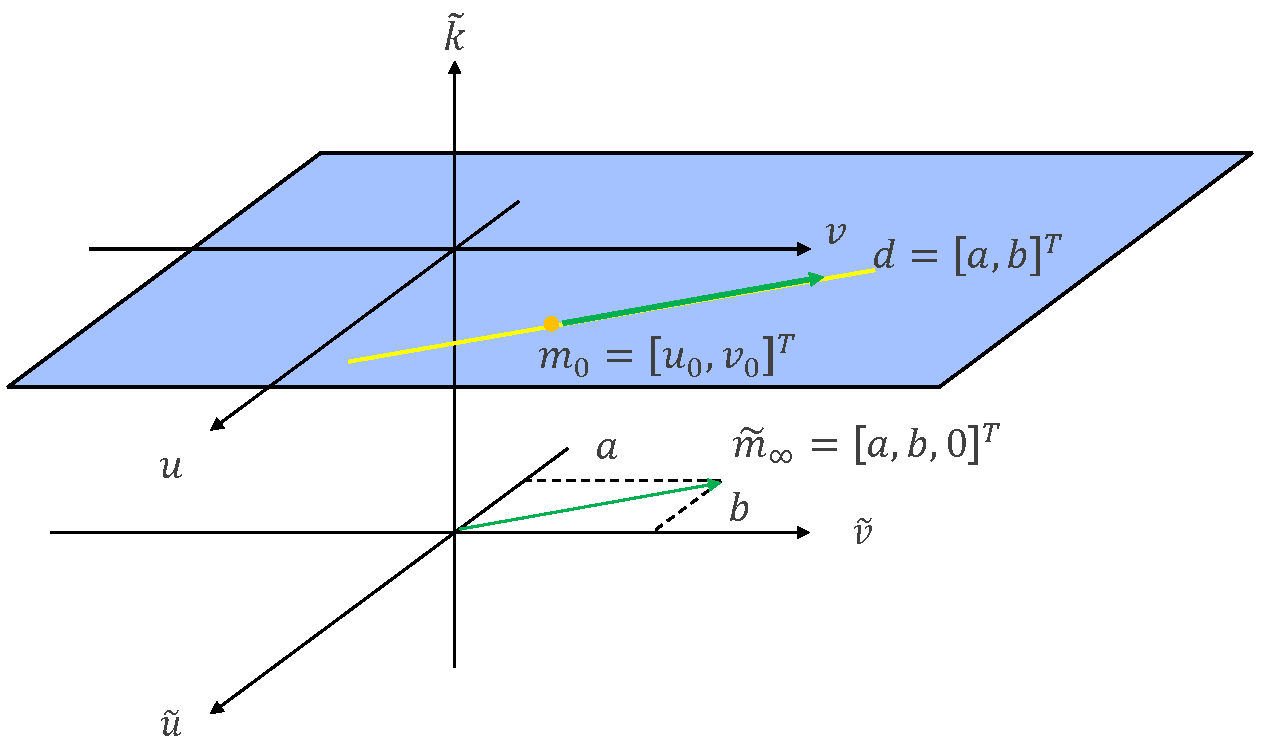
\includegraphics[width=0.6\linewidth]{./img/_projective_point_inifinity.pdf}
            \caption{Example of infinity point in $\mathbb{P}^2$}
        \end{figure}

        In 3D, the definition is trivially extended as:
        \[ 
            \tilde{\vec{M}}_\infty = 
            \lim_{\lambda \rightarrow \infty} \begin{pmatrix} \frac{x_0}{\lambda} + a \\ \frac{y_0}{\lambda} + b \\ \frac{z_0}{\lambda} + c \\ \frac{1}{\lambda} \end{pmatrix} \equiv
            \begin{pmatrix} a \\ b \\ c \\ 0 \end{pmatrix}
        \]

    \item[Perspective projection] \marginnote{Perspective projection in projective space}
        Given a point $\vec{M}_C = (x_C, y_C, z_C)$ in the CRF and its corresponding point $\vec{m} = (u, v)$ in the image,
        the non-linear perspective projection in Euclidean space can be done linearly in the projective space as:
        \[  
            \begin{split}
                \tilde{\vec{m}} &\equiv 
                \begin{pmatrix} u \\ v \\ 1 \end{pmatrix} \equiv
                \begin{pmatrix} f_u\frac{x_C}{z_C} + u_0 \\ f_v\frac{y_C}{z_C} +v_0 \\ 1 \end{pmatrix} \equiv
                z_C \begin{pmatrix} f_u\frac{x_C}{z_C} + u_0 \\ f_v\frac{y_C}{z_C} +v_0 \\ 1 \end{pmatrix} \\
                &\equiv \begin{pmatrix} f_u x_C + z_C u_0 \\ f_v y_C + z_C v_0 \\ z_C \end{pmatrix} \equiv
                \begin{pmatrix} f_u & 0 & u_0 & 0 \\ 0 & f_v & v_0 & 0 \\ 0 & 0 & 1 & 0 \end{pmatrix} \begin{pmatrix} x_C \\ y_C \\ z_C \\ 1 \end{pmatrix} \equiv
                \matr{P}_\text{int} \tilde{\vec{M}}_C
            \end{split}
        \]

        \begin{remark}
            The equation can be written to take account of the arbitrary scale factor $k$ as:
            \[ k\tilde{\vec{m}} = \matr{P}_\text{int} \tilde{\vec{M}}_C \]
            or, if $k$ is omitted, as:
            \[ \tilde{\vec{m}} \approx \matr{P}_\text{int} \tilde{\vec{M}}_C \]
        \end{remark}

        \begin{remark}
            In projective space, we can also project in Euclidean space the point at infinity of parallel 3D lines in CRF with direction $(a, b, c)$:
            \[ 
                \tilde{\vec{m}}_\infty \equiv 
                    \matr{P}_\text{int} \begin{pmatrix} a \\ b \\ c \\ 0 \end{pmatrix} \equiv
                    \begin{pmatrix} f_u & 0 & u_0 & 0 \\ 0 & f_v & v_0 & 0 \\ 0 & 0 & 1 & 0 \end{pmatrix} \begin{pmatrix} a \\ b \\ c \\ 0 \end{pmatrix} \equiv
                    \begin{pmatrix} f_u a + c u_0 \\ f_v b + c v_0 \\ c \end{pmatrix} \equiv
                    c\begin{pmatrix} f_u \frac{a}{c} + u_0 \\ f_v \frac{b}{c} + v_0 \\ 1 \end{pmatrix}
            \]
            Therefore, the Euclidean coordinates are:
            \[ \vec{m}_\infty = \begin{pmatrix} f_u \frac{a}{c} + u_0 \\ f_v \frac{b}{c} + v_0 \end{pmatrix} \]
            
            Note that this is not possible when $c = 0$.
        \end{remark}
\end{description}